\mysection{Distribuované algoritmy}

Vlastnosti modelu:
\begin{itemize}
    \item niekoľko počítačov zapojených do siete obojsmernými linkami
    \item majú jednoznačné id, komunikujú len správami
    \item správy sa nestrácajú, nemenia poradie, ale môže im to trvať ľubovoľne dlho -- asynchrónna
    komunikácia
\end{itemize}

Ciele:
\begin{itemize}
    \item poslať čo najmenej správ
    \item minimalizovať dobu behu algoritmu
\end{itemize}


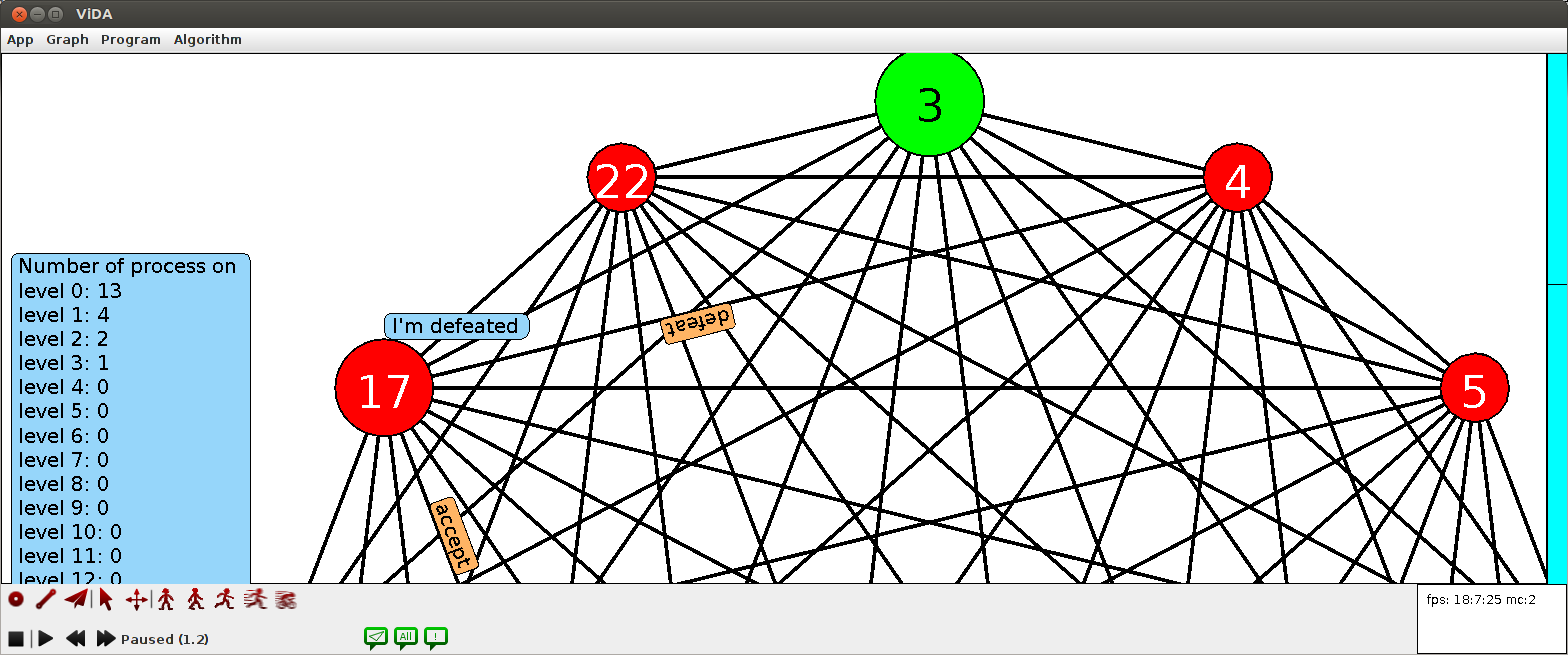
\includegraphics[width=\columnwidth]{le}

\mysection{Navizualizované algoritmy}

\begin{itemize}

    \item broadcast -- \textit{ako povedať novú klebetu všetkým v sieti?}
    \item traverzovanie -- \textit{ako len s pomocou jednej správy prehľadať celý graf?}
    \item voľba šéfa na úplnom grafe -- \textit{ako sa spomedzi niekoľkých identických programov
    dá zvoliť jeden šéf? a čo ak pri tom chceme poslať čo najmenej správ?}

\end{itemize}

\noindent
\begin{figure*}
\centering
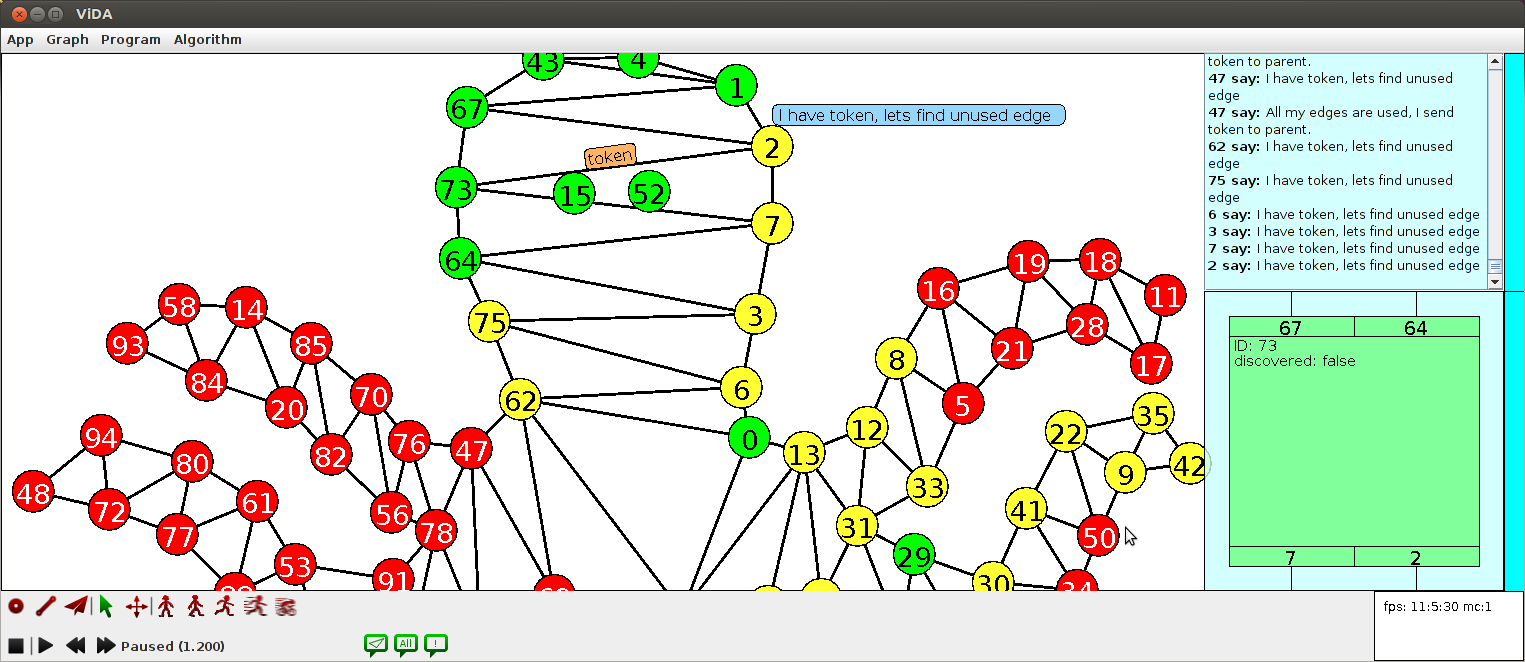
\includegraphics[width=\columnwidth]{traverz}
\caption{\emph{traverzovanie} -- graf sa prehľadáva pomocou jedinej správy -- \emph{tokenu}. Zelené vrcholy
sú nenavštívené, oranžové sú navštívené, červené sú úplne vybavené -- už preskúmali všetkých susedov}
\label{img:historia} 
\end{figure*}

    
\mysection{Nástroje}

\begin{itemize}
    \item úprava grafu
    \begin{itemize}
        \item pridávanie, mazanie, editovanie, hýbanie vrcholov a hrán
        \item ukladanie, automatické generovanie rôznych typov a veľkostí
        \item verifikácia -- napr. niektoré algoritmy sú určené len pre úplné grafy
    \end{itemize}
    \item časovanie správ
    \begin{itemize}
        \item možnosť chytiť správu a presunúť ju na iné miesto na hrane
        \item nastavovanie rýchlostí hrán, správ
    \end{itemize}
    \item selekcia -- zobrazovanie dodatočných informácií
    \item plánujú sa mnohé ďalšie


\end{itemize}



%TODO aplikacia pred spustenim programu


\mysection{Spôsob vizualizácie}

\begin{itemize}

    \item 
    \item informácie priamo v grafe -- intuitívne spojenie vizuálnych a hodnotových
    vlastností, napr. veľkosť vrchola = level, farba vrchola = stav (napr. červený =
    mŕtvy/porazený/neaktívny)
    \item zobrazovanie udalostí priamo v grafe -- netreba vrtieť hlavou a hľadať, čo sa kde deje,
    informácie sa zobrazujú tam, kde sa ich to týka, všetko pomocou \emph{vyskakovacích bubliniek}
    \item interaktivita -- \emph{čo by sa stalo, keď\dots?} užívateľ môže priamo ovplyvňovať, čo sa
    stane
    \item detekcia a vystevlenie zaujímavých udalostí -- keď sa niečo stane, aplikácia sa pozastaví a vysvetlí
    \emph{čo sa stalo? prečo sa to stalo? kde sa to stalo? čo sa bude diať ďalej?}

\end{itemize}

%TODO zobrazovanie informacii za behu

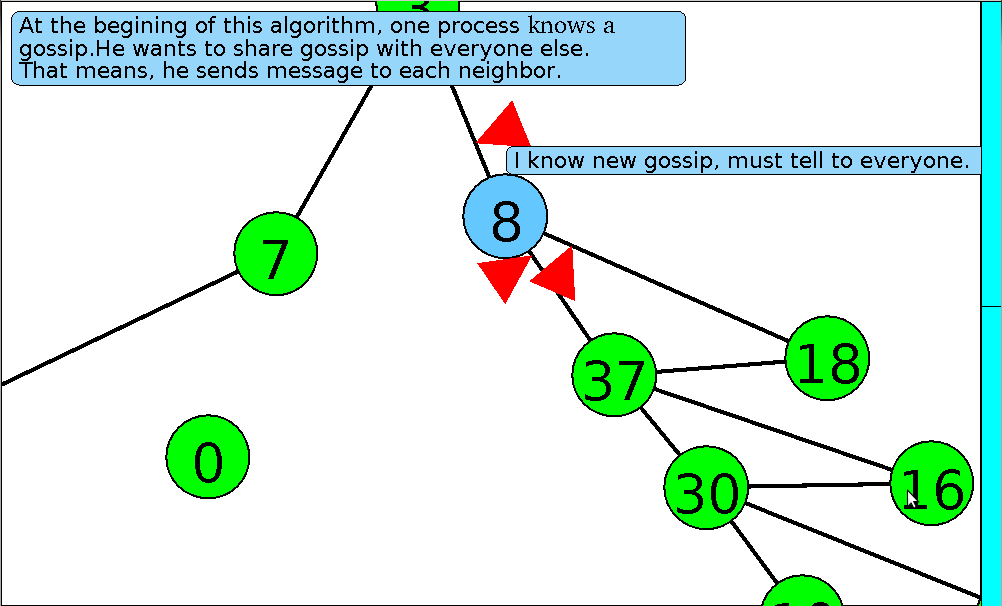
\includegraphics[width=\columnwidth]{bfs}

\mysection{C}

%TODO popis konkretnych algoritmov

\mysection{Plány do budúcnosti}


\begin{itemize}
    \item ďalšie algoritmy
    \begin{itemize}
        \item GHS -- \emph{voľba šéfa na všeobecnom grafe}
        \item KKM -- \emph{voľba šéfa s využitím traverzovania}
        \item routing -- \emph{smerovanie dát v sieti. Kam poslať paket, aby sa dostal do cieľa?}
        \item problém dohody
    \end{itemize}
    \item viac zábavy, viac interaktivity -- \emph{užívateľ sa môže zahrať na zákeráka a snažiť sa
    donútiť algoritmus, aby poslal čo najviac správ}
    \item viacero programovacích jazykov, viac nástrojov pre vizualizáciu
\end{itemize}

%TODO plany do buducnosti
